\section{Generating the Running Example} \label{sec:exp-tabu}
In this section we will use our Tabu Search to generate a configuration that shares similarities to our running example, which can be seen in \cref{fig:running-example} and found in \cref{sec:runningexample}. We will use the same modules that are included in the running example to optimize an initial linear configuration. We will optimize the configuration such that it is able to produce items of the recipes described in \cref{fig:toy-recipes} as fast as possible. Then we will compare the configuration generated through our tabu search to the running example, which we made by hand.

\subsection{The Configuration Found by the Tabu Search}
As mentioned, our total set of modules for the tabu search will be the modules seen in \cref{fig:running-example}. Furthermore, we wish to optimize for an order asking to produce 3 items for each recipe described in \cref{fig:toy-recipes}. This is done in the hopes that 3 items of each recipe is enough to satiate the configuration enough, such that it encourages parallelization transformations. The resulting configuration of the tabu search can be seen in \cref{fig:tabu-config}.

\begin{figure}[H]
	\centering
	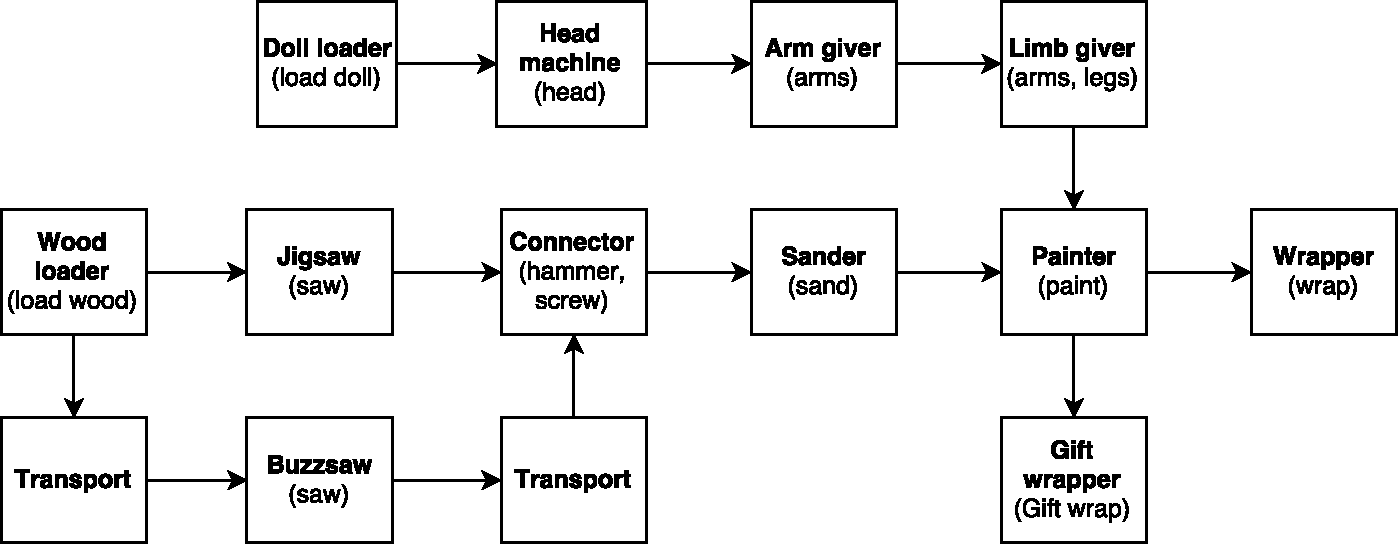
\includegraphics[width=.8\textwidth]{tabu-config.pdf}
	\caption{The configuration generated by our tabu search.}
	\label{fig:tabu-config}
\end{figure}

This configuration generated by our tabu search shows promise, as it has both utilized our anti-serialization and parallelization rules and is somewhat similar to the running example. 

We can see that it has used the anti-serialization rules because of the modules that uniquely only produce work for the doll recipe, are disconnected from the rest of the configuration. With the branches joining and splitting from the configuration at the common module \texttt{Painter}. In general, our tabu search has anti-serialized much in the same way as we did, when we made \cref{fig:running-example} by hand. The only exception is that we connected the modules \texttt{Sander} and \texttt{Wrapper} through a transport module, this being done so that rocking horse items may avoid going through \texttt{Painter}. We however have not made any type of transformation rule that would be allow the tabu search to do this. 

We can see that the search has used parallelization rules, as we have two paths from \texttt{Wood Loader} to \texttt{Connector} that both can do the work $saw$. This is different from the running example, as we there had the modules \texttt{Jigsaw} and \texttt{Buzzsaw} placed next to each other instead of parallel. In our UPPAAL model, an item can not pass through a module that can perform work on it. Thus we have not set up a transformation rule, which would place \textit{Jigsaw} and \textit{Buzzsaw} next to each other. If run on our model, all the work $saw$ would simply be done on the first module, and the second would function merely as a glorified transport module.

A genuine advantage that the running example has over the configuration, we found with our tabu search, is that it parallelized the modules \texttt{Arm Giver} and \texttt{Leg Giver} with \texttt{Limb Giver}. This was not possible for our tabu search, as our parallelization rules describe that the parallization must be a single module capable of all the active work that the original module is doing. It can not be a set of modules that together are able to perform all the original module's active work. Of course in reality, this type of parallelizatiion could be beneficial, as is the case in the running example.

Overall we are satisfied by the outcome that is our tabu search, as it seems capable, at least for this example, to heuristically find optimized solutions.
